\documentclass[11pt]{article}
\usepackage{tikz}

\makeatletter
% Define the stub radius parameter
\pgfkeys{
  /tikz/stub radius/.initial=5pt,
  /tikz/stub radius/.default=5pt
}

% Assume these registers and macro exist
\newdimen\my@N  % North (top) y coordinate
\newdimen\my@E  % East (right) x coordinate
\newdimen\my@W  % West (left) x coordinate
\newdimen\my@S  % South (bottom) y coordinate
\newdimen\my@Cx % Center x coordinate
\newdimen\my@Cy % Center y coordinate
\newdimen\my@halfwidth
\newdimen\my@halfheight
\newdimen\my@stubradius

% Macro to set NESW coordinates from southwest/northeast
\def\setmy@NEWSC{%
  \southwest
  \my@W=\pgf@x%
  \my@S=\pgf@y%
  \northeast
  \my@E=\pgf@x%
  \my@N=\pgf@y%
  % Calculate center
  \my@Cx=.5\my@W%
  \advance\my@Cx by.5\my@E%
  \my@Cy=.5\my@S%
  \advance\my@Cy by.5\my@N%
  % Calculate half dimensions
  \my@halfwidth=\my@E%
  \advance\my@halfwidth by-\my@W%
  \my@halfwidth=.5\my@halfwidth%
  \my@halfheight=\my@N%
  \advance\my@halfheight by-\my@S%
  \my@halfheight=.5\my@halfheight%
}

\pgfdeclareshape{stub rectangle}{%
  % Inherit anchors from rectangle
  \inheritsavedanchors[from=rectangle]
  \inheritanchor[from=rectangle]{center}
  \inheritanchor[from=rectangle]{north}
  \inheritanchor[from=rectangle]{south}
  \inheritanchor[from=rectangle]{east}
  \inheritanchor[from=rectangle]{west}
  \inheritanchor[from=rectangle]{north east}
  \inheritanchor[from=rectangle]{north west}
  \inheritanchor[from=rectangle]{south east}
  \inheritanchor[from=rectangle]{south west}
  
  % Background path
  \backgroundpath{%
    % Get NESW coordinates
    \setmy@NEWSC
    % Get stub radius
    \pgfmathsetlength\my@stubradius{\pgfkeysvalueof{/tikz/stub radius}}%
    % Check if stub radius is too large
    \ifdim\my@stubradius>\my@halfwidth
      \pgferror{stub radius (\the\my@stubradius) is larger than half the width (\the\my@halfwidth)}%
    \fi
    \ifdim\my@stubradius>\my@halfheight
      \pgferror{stub radius (\the\my@stubradius) is larger than half the height (\the\my@halfheight)}%
    \fi
    % Draw the path with cut corners
    % Start at bottom edge, after SW corner bite
    \pgfpathmoveto{\pgfpoint{\my@W+\my@stubradius}{\my@S}}%
    % Line to SE corner bite start
    \pgfpathlineto{\pgfpoint{\my@E-\my@stubradius}{\my@S}}%
    % SE corner arc: we're west of corner, need to go north
    % Arc goes counterclockwise from current position
    \pgfpatharc{180}{90}{\my@stubradius}%
    % Now at radius north of SE corner
    % Line to NE corner bite start
    \pgfpathlineto{\pgfpoint{\my@E}{\my@N-\my@stubradius}}%
    % NE corner arc: we're south of corner, need to go west
    \pgfpatharc{270}{180}{\my@stubradius}%
    % Now at radius west of NE corner
    % Line to NW corner bite start
    \pgfpathlineto{\pgfpoint{\my@W+\my@stubradius}{\my@N}}%
    % NW corner arc: we're east of corner, need to go south
    \pgfpatharc{0}{-90}{\my@stubradius}%
    % Now at radius south of NW corner
    % Line to SW corner bite start
    \pgfpathlineto{\pgfpoint{\my@W}{\my@S+\my@stubradius}}%
    % SW corner arc: we're north of corner, need to go east
    \pgfpatharc{90}{0}{\my@stubradius}%
    % Now back at starting point
    \pgfpathclose%
  }
}
\makeatother

\begin{document}

% Test with default stub radius
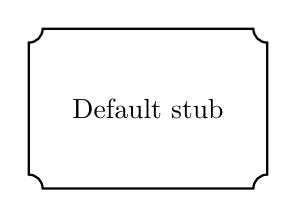
\begin{tikzpicture}
  \node[stub rectangle, draw, thick, minimum width=3cm, minimum height=2cm] at (0,0) {Default stub};
\end{tikzpicture}

\vspace{1cm}

% Test with different stub radii
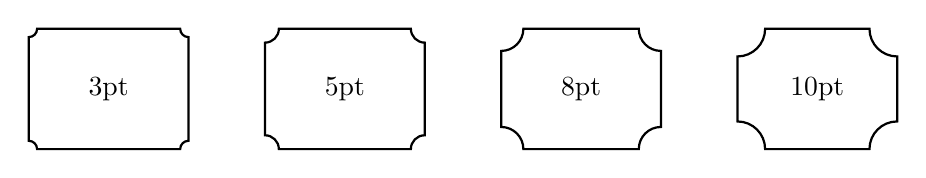
\begin{tikzpicture}
  \node[stub rectangle, stub radius=3pt, draw, thick, minimum width=2cm, minimum height=1.5cm] at (0,0) {3pt};
  \node[stub rectangle, stub radius=5pt, draw, thick, minimum width=2cm, minimum height=1.5cm] at (3,0) {5pt};
  \node[stub rectangle, stub radius=8pt, draw, thick, minimum width=2cm, minimum height=1.5cm] at (6,0) {8pt};
  \node[stub rectangle, stub radius=10pt, draw, thick, minimum width=2cm, minimum height=1.5cm] at (9,0) {10pt};
\end{tikzpicture}

\vspace{1cm}

% Test with styling
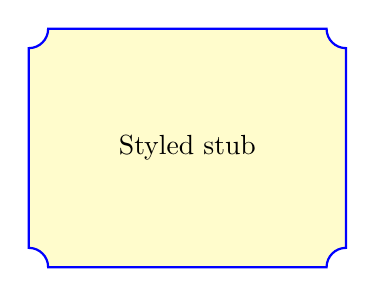
\begin{tikzpicture}
  \node[stub rectangle, stub radius=7pt, draw=blue, thick, fill=yellow!20, minimum width=4cm, minimum height=3cm] at (0,0) {Styled stub};
\end{tikzpicture}

% Test error condition (commented out to avoid compilation error)
% \begin{tikzpicture}
%   \node[stub rectangle, stub radius=2cm, draw, minimum width=2cm, minimum height=1cm] at (0,0) {Too big};
% \end{tikzpicture}

\end{document}

\documentclass[11pt]{article}
\usepackage{tikz}

\makeatletter
% Define the stub radius parameter
\pgfkeys{
  /tikz/stub radius/.initial=5pt,
  /tikz/stub radius/.default=5pt
}

% Assume these registers and macro exist
\newdimen\my@N  % North (top) y coordinate
\newdimen\my@E  % East (right) x coordinate
\newdimen\my@W  % West (left) x coordinate
\newdimen\my@S  % South (bottom) y coordinate
\newdimen\my@Cx % Center x coordinate
\newdimen\my@Cy % Center y coordinate
\newdimen\my@halfwidth
\newdimen\my@halfheight
\newdimen\my@stubradius

% Macro to set NESW coordinates from southwest/northeast
\def\setmy@NEWSC{%
  \southwest
  \my@W=\pgf@x%
  \my@S=\pgf@y%
  \northeast
  \my@E=\pgf@x%
  \my@N=\pgf@y%
  % Calculate center
  \my@Cx=.5\my@W%
  \advance\my@Cx by.5\my@E%
  \my@Cy=.5\my@S%
  \advance\my@Cy by.5\my@N%
  % Calculate half dimensions
  \my@halfwidth=\my@E%
  \advance\my@halfwidth by-\my@W%
  \my@halfwidth=.5\my@halfwidth%
  \my@halfheight=\my@N%
  \advance\my@halfheight by-\my@S%
  \my@halfheight=.5\my@halfheight%
}

\pgfdeclareshape{stub rectangle}{%
  % Inherit anchors from rectangle
  \inheritsavedanchors[from=rectangle]
  \inheritanchor[from=rectangle]{center}
  \inheritanchor[from=rectangle]{north}
  \inheritanchor[from=rectangle]{south}
  \inheritanchor[from=rectangle]{east}
  \inheritanchor[from=rectangle]{west}
  \inheritanchor[from=rectangle]{north east}
  \inheritanchor[from=rectangle]{north west}
  \inheritanchor[from=rectangle]{south east}
  \inheritanchor[from=rectangle]{south west}
  
  % Background path
  \backgroundpath{%
    % Get NESW coordinates
    \setmy@NEWSC
    % Get stub radius
    \pgfmathsetlength\my@stubradius{\pgfkeysvalueof{/tikz/stub radius}}%
    % Check if stub radius is too large
    \ifdim\my@stubradius>\my@halfwidth
      \pgferror{stub radius (\the\my@stubradius) is larger than half the width (\the\my@halfwidth)}%
    \fi
    \ifdim\my@stubradius>\my@halfheight
      \pgferror{stub radius (\the\my@stubradius) is larger than half the height (\the\my@halfheight)}%
    \fi
    % Draw the path with cut corners
    % Start at bottom left, after the stub
    \pgfpathmoveto{\pgfpoint{\my@W+\my@stubradius}{\my@S}}%
    % Line to bottom right stub start
    \pgfpathlineto{\pgfpoint{\my@E-\my@stubradius}{\my@S}}%
    % Arc for bottom right corner (from 270 to 0 degrees)
    \pgfpatharc{270}{0}{\my@stubradius}%
    % Line to top right stub start
    \pgfpathlineto{\pgfpoint{\my@E}{\my@N-\my@stubradius}}%
    % Arc for top right corner (from 0 to 90 degrees)
    \pgfpatharc{0}{90}{\my@stubradius}%
    % Line to top left stub start
    \pgfpathlineto{\pgfpoint{\my@W+\my@stubradius}{\my@N}}%
    % Arc for top left corner (from 90 to 180 degrees)
    \pgfpatharc{90}{180}{\my@stubradius}%
    % Line to bottom left stub start
    \pgfpathlineto{\pgfpoint{\my@W}{\my@S+\my@stubradius}}%
    % Arc for bottom left corner (from 180 to 270 degrees)
    \pgfpatharc{180}{270}{\my@stubradius}%
    % Close the path
    \pgfpathclose%
  }
}
\makeatother

\begin{document}

% Test with default stub radius
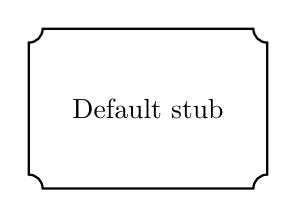
\begin{tikzpicture}
  \node[stub rectangle, draw, thick, minimum width=3cm, minimum height=2cm] at (0,0) {Default stub};
\end{tikzpicture}

\vspace{1cm}

% Test with different stub radii
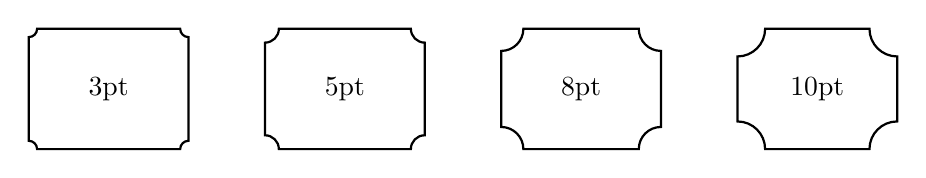
\begin{tikzpicture}
  \node[stub rectangle, stub radius=3pt, draw, thick, minimum width=2cm, minimum height=1.5cm] at (0,0) {3pt};
  \node[stub rectangle, stub radius=5pt, draw, thick, minimum width=2cm, minimum height=1.5cm] at (3,0) {5pt};
  \node[stub rectangle, stub radius=8pt, draw, thick, minimum width=2cm, minimum height=1.5cm] at (6,0) {8pt};
  \node[stub rectangle, stub radius=10pt, draw, thick, minimum width=2cm, minimum height=1.5cm] at (9,0) {10pt};
\end{tikzpicture}

\vspace{1cm}

% Test with styling
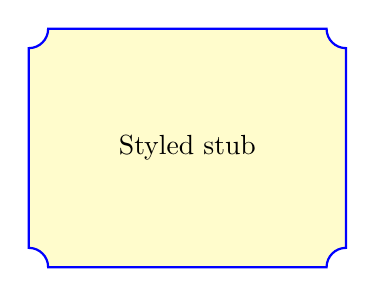
\begin{tikzpicture}
  \node[stub rectangle, stub radius=7pt, draw=blue, thick, fill=yellow!20, minimum width=4cm, minimum height=3cm] at (0,0) {Styled stub};
\end{tikzpicture}

% Test error condition (commented out to avoid compilation error)
% \begin{tikzpicture}
%   \node[stub rectangle, stub radius=2cm, draw, minimum width=2cm, minimum height=1cm] at (0,0) {Too big};
% \end{tikzpicture}

\end{document}
